\section{二项分布与超几何分布}

本节要点:
\begin{itemize}
    \item 掌握二项分布及其意义;
    \item 掌握超几何分布及其意义。
\end{itemize}

%============================================================
\subsection{二项分布}

{\bf 二项分布}又称{\bf 伯努利分布},记作$B\left( n,p \right) $,因其分布律表达式中包含二项式系数而得名,描述$n$重伯努利试验中具有发生概率$p$的事件发生$x$次的概率的分布规律:
\[
P\left\{ X=x \right\} =C_{n}^{x}p^x\left( 1-p \right) ^{n-x},\qquad \begin{array}{l}
	x=0,1,\cdots ,n\\
	p\in \left( 0,1 \right)\\
\end{array}
\]
其中:
\begin{itemize}
    \item $x$:表示事件发生的次数,包括一次也不发生($x=0$)和每次都发生($x=n$);
    \item $p$:表示事件发生的概率;
    \item $C_{n}^{x}$:$n$次子试验中,事件发生了$x$次的次数,注意,这里用组合,表示我们只关心$x$次,而不关心具体是哪$x$次;
    \item $p^x$:表示事件发生$x$次的概率;
    \item $\left( 1-p \right) ^{n-x}$:表示其余$n-x$次子试验中事件不发生的概率。
\end{itemize}
伯努利试验中,小概率事件倾向于少发生,大概率事件倾向于多次发生,且发生概率最大的在$np$次。

\begin{figure}[h]
\centering
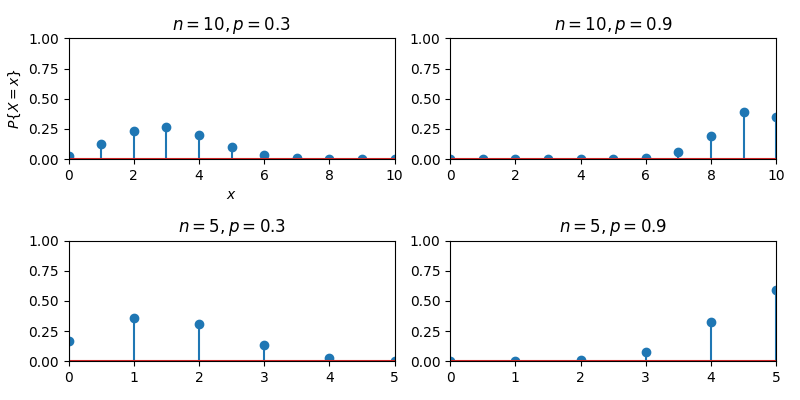
\includegraphics[height=4cm]{7.4-1.png}
\caption{二项分布}
\end{figure}

\begin{tcolorbox}
二项分布描述伯努利试验,我们可以知道在固定$n$次子试验中,事件$A$发生几次的概率是最大的。最典型的应用就是$n$次放回抽样,计算抽到$x$个次品的概率。
\end{tcolorbox}

%============================================================
\subsection{超几何分布}

{\bf 超几何分布},记作$H\left( M,N,n \right) $,因其分布律与超几何函数的级数展开式的系数类似而得名,描述不放回抽取试验,从$N$个样品中抽取$n$个,出现$x$个次品的概率分布:
\[
P\left\{ X=x \right\} =\frac{C_{N-M}^{n-x}C_{M}^{x}}{C_{N}^{n}}, \begin{array}{l}
	N>1,M\leqslant N\\
	n\leqslant N,x\in \left[ \max \left\{ 0,M+n-N \right\} ,\min \left\{ M,n \right\} \right]\\
\end{array}
\]
其中:
\begin{itemize}
    \item $N,M$:共$N$个样品,其中有$M$个次品;
    \item $n,x$:抽取$n$个,其中$x$个为次品。
\end{itemize}
超几何分布中,抽到$\frac{M}{N}\cdot n$的概率最大。

\begin{figure}[h]
\centering
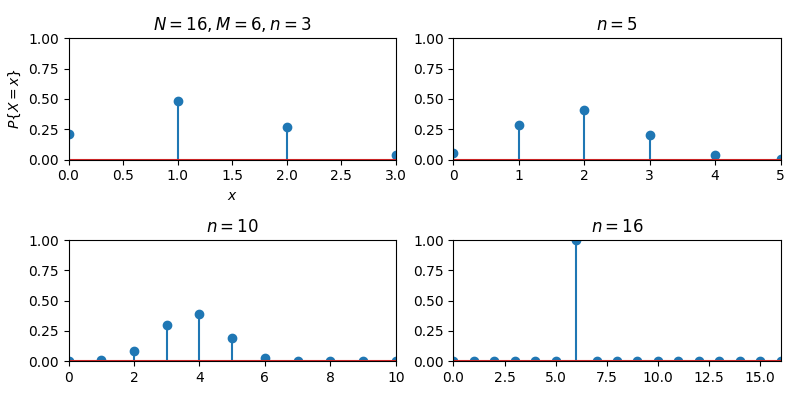
\includegraphics[height=4cm]{7.4-2.png}
\caption{超几何分布,16个样品,6个次品}
\end{figure}
\begin{figure}[h]
\centering
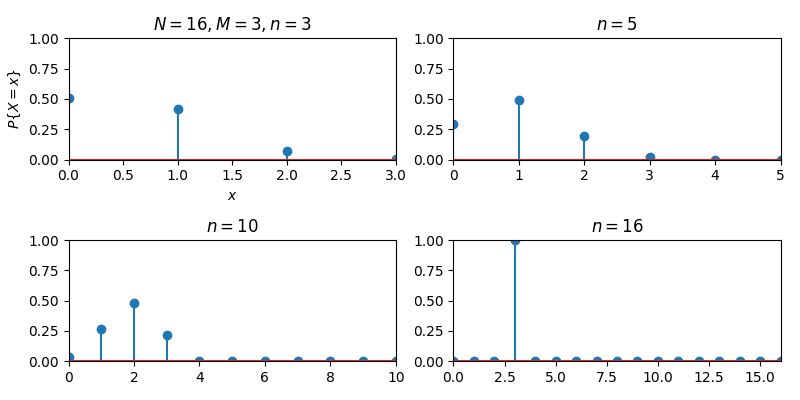
\includegraphics[height=4cm]{7.4-3.png}
\caption{超几何分布,16个样品,3个次品}
\end{figure}

\begin{tcolorbox}
超几何分布描述“不放回”抽取试验,不是基于伯努利试验,描述抽到$x$个次品的概率分布。
\end{tcolorbox}

%============================================================
\subsection{习题}

\begin{example}[综合运用7,难度:$\star $]
一个车间有3台车床,它们各自独立工作。设在一段时间内发生故障的车床数为$X$,在下列两种情形下分别求$X$的分布列。
\begin{enumerate}
    \item 假设这3台车床型号相同,它们发生故障的概率都是20\%;
    \item 这3台车床中有A型号2台,B型号1台,A型车床发生故障的概率为10\%,B型车床发生故障的概率为20\%。
\end{enumerate}
\end{example}

解:

(1)典型的二项分布:
\begin{align*}
&P\left\{ X=0 \right\} =C_{3}^{0}\cdot 0.2^0\cdot \left( 1-0.2 \right) ^{3-0}=0.512 \\
&P\left\{ X=1 \right\} =C_{3}^{1}\cdot 0.2^1\cdot \left( 1-0.2 \right) ^{3-1}=0.384 \\
&P\left\{ X=2 \right\} =C_{3}^{2}\cdot 0.2^2\cdot \left( 1-0.2 \right) ^{3-2}=0.096 \\
&P\left\{ X=3 \right\} =C_{3}^{3}\cdot 0.2^3\cdot \left( 1-0.2 \right) ^{3-3}=0.008
\end{align*}

(2)不是二项分布,需要分别计算:
\begin{align*}
P\left\{ X=0 \right\} &=\left( 1-0.1 \right) \cdot \left( 1-0.1 \right) \cdot \left( 1-0.2 \right) =0.648 \\
P\left\{ X=1 \right\} &=0.1\cdot \left( 1-0.1 \right) \cdot \left( 1-0.2 \right) \\
&+\left( 1-0.1 \right) \cdot 0.1\cdot \left( 1-0.2 \right) +\left( 1-0.1 \right) \cdot \left( 1-0.1 \right) \cdot 0.2=0.306 \\
P\left\{ X=2 \right\} &=0.1\cdot 0.1\cdot \left( 1-0.2 \right) +0.1\cdot \left( 1-0.1 \right) \cdot 0.2+\left( 1-0.1 \right) \cdot 0.1\cdot 0.2 \\
&=0.044 \\
P\left\{ X=3 \right\} &=0.1\cdot 0.1\cdot 0.2=0.002
\end{align*}

\begin{tcolorbox}
本题考察二项分布的概念,没有难度。
\end{tcolorbox}

~

\begin{example}[拓广探索8,难度:$\star \star \star $]
某药厂研制一种新药,宣称对治疗某种疾病的有效率为90\%,随机选择了10名患者,经过使用该药治疗后,治愈的人数不超过6人,你是否怀疑药厂的宣传?
\end{example}

解:

假设新药的有效率90\%为真,则治愈人数不超过6人的概率:
\begin{align*}
&P\left\{ X=0 \right\} =C_{10}^{0}\cdot 0.9^0\cdot \left( 1-0.9 \right) ^{10-0}=1\times 10^{-10} \\
&P\left\{ X=1 \right\} =C_{10}^{1}\cdot 0.9^1\cdot \left( 1-0.9 \right) ^{10-1}=9\times 10^{-9} \\
&P\left\{ X=2 \right\} =C_{10}^{2}\cdot 0.9^2\cdot \left( 1-0.9 \right) ^{10-2}=3.645\times 10^{-7} \\
&P\left\{ X=3 \right\} =C_{10}^{3}\cdot 0.9^3\cdot \left( 1-0.9 \right) ^{10-3}=8.748\times 10^{-6} \\
&P\left\{ X=4 \right\} =C_{10}^{4}\cdot 0.9^4\cdot \left( 1-0.9 \right) ^{10-4}=0.000137781 \\
&P\left\{ X=5 \right\} =C_{10}^{5}\cdot 0.9^5\cdot \left( 1-0.9 \right) ^{10-5}=0.00148803 \\
&P\left\{ X=6 \right\} =C_{10}^{6}\cdot 0.9^6\cdot \left( 1-0.9 \right) ^{10-6}=0.0111603 \\
&\sum_{i=0}^6{P\left\{ X=i \right\}}=0.0127952
\end{align*}
也即在有效率90\%的情况下治愈人数不超过6人的概率仅为仅为1.28\%,显然这个有效率90\%是小概率事件,有理由怀疑宣传的真实性。

\begin{tcolorbox}
本题是数理统计的检验假设问题,稍微有点超纲。
\end{tcolorbox}




